\documentclass[conference]{IEEEtran}
\usepackage{graphicx,booktabs,amsmath,url,flushend}
\begin{document}
\title{Machine Learning for Spatial Enhancement of PM$_{2.5}$ Prediction over India}
\author{\IEEEauthorblockN{Harsh Meshram, Chandranil Das, Dhrubojyoti Saha, Dineshwar Okram, Tanuj Singh}\IEEEauthorblockA{Group 1, Project 3, EE708\\Indian Institute of Technology Kanpur, India}}
\maketitle
\begin{abstract}
We estimate daily CAMS PM$_{2.5}$ over India during 2020--2024 from aerosol and meteorological predictors. A spatial block split withholds 112 of 494 locations across all dates. Random forest (RF) achieves RMSE 31.89~$\mu$g/m$^3$ and $R^2=0.742$, compared with 35.34 and 0.683 for inverse distance weighting (IDW). Interpolated predictors generate exploratory 0.25$^\circ$ maps. Evaluation establishes agreement with CAMS at withheld coarse-grid locations, but does not establish fine-scale accuracy or agreement with ground measurements.
\end{abstract}
\begin{IEEEkeywords}PM$_{2.5}$, CAMS EAC4, random forest, spatial validation\end{IEEEkeywords}
\section{Objective and Data}
The objective is to estimate CAMS PM$_{2.5}$ from atmospheric conditions, compare ML with interpolation, identify important predictors, assess regional and seasonal performance, and produce finer maps. CAMS EAC4 reanalysis supplies variables on a 0.75$^\circ$ grid~\cite{cams}. The processed table contains 902,538 records: 494 India locations over 1,827 days, 1 January 2020 to 31 December 2024.

The target is near-surface PM$_{2.5}$. Nine inputs are aerosol optical depth at 550~nm (AOD), 10~m wind components, 2~m temperature and dewpoint, surface pressure, latitude, longitude and month. All atmospheric inputs and targets originate from CAMS. Regions are IGP, northwest, central, south, northeast and Himalaya.
\section{Preprocessing and Spatial Evaluation}
The preparation script concatenates 60 monthly files and averages 3-hourly samples by day. PM$_{2.5}$ is multiplied by $10^9$ to convert kg/m$^3$ to $\mu$g/m$^3$; temperatures become Celsius and pressure hPa. A supplied India mask and regional labels select cells. The processed CSV has no missing values or duplicate date--location keys. Raw subdaily completeness was not independently audited. Seasons are Jan--Feb, Mar--May, Jun--Sep and Oct--Dec.

Locations are grouped into 5-by-5 blocks on the native grid. Blocks satisfying $(r+2c)\bmod 5=0$ form the spatial test. There are 382 training cells (697,914 records) and 112 test cells (204,624 records). All days of each cell remain together. Regional test shares range from 12\% to 28\%. Block boundaries do not enforce a minimum train--test distance. The held-out spatial test provides the validation assessment; there is no separate tuning set or future-year evaluation.
\section{Model Architecture and Baselines}
\textbf{Linear regression} fits one global linear relationship. \textbf{Random forest} averages 100 regression trees~\cite{breiman,sklearn}, with bootstrap sampling, minimum 10 samples per leaf, all features considered at each split, and seed 42. No explicit depth cap or physics constraint is imposed. Both models fit training locations only.

\textbf{IDW} predicts a withheld location from same-day PM$_{2.5}$ at its eight nearest training cells:
\begin{equation}
\hat y(s,t)=\frac{\sum_{i\in N_8(s)}d(s,s_i)^{-2}y(s_i,t)}{\sum_{i\in N_8(s)}d(s,s_i)^{-2}}.
\end{equation}
Distances use latitude--longitude degrees, an approximation that neglects latitude-dependent physical distance. IDW uses nearby target values; ML uses atmospheric predictors at the test cell. The information available to the methods therefore differs.
\section{Performance and Model Efficiency}
Metrics retain all extremes and negative predictions. Table~\ref{tab:overall} reports pooled spatial test scores. RF reduces RMSE by 9.8\% and MAE by 12.8\% relative to IDW. RF training RMSE, MAE and $R^2$ are 18.85, 8.47 and 0.915. Training scores are resubstitution scores; the held-out $R^2$ of 0.742 shows a generalization gap.
\begin{table}[t]\caption{Held-out scores. Errors and bias in $\mu$g/m$^3$.}\label{tab:overall}\centering
\begin{tabular}{lrrrr}\toprule Method&RMSE&MAE&$R^2$&Bias\\\midrule
IDW&35.34&20.43&0.683&$-6.75$\\
Linear regression&46.72&32.14&0.446&$-12.88$\\
Random forest&\textbf{31.89}&\textbf{17.82}&\textbf{0.742}&$-5.58$\\\bottomrule\end{tabular}\end{table}

RF outperforms IDW in four regions. RF/IDW $R^2$ values are central 0.752/0.696, Himalaya 0.784/0.457, IGP 0.538/0.556, northeast 0.738/$-0.740$, northwest 0.748/0.805 and south 0.474/0.451. RF wins in every season, with $R^2$ 0.690 (winter), 0.601 (pre-monsoon), 0.805 (monsoon) and 0.715 (post-monsoon).

Impurity importance ranks AOD (0.305), pressure (0.193) and temperature (0.137) highest. Importance describes model use rather than causal atmospheric influence. Correlated predictors and shared CAMS provenance limit interpretation. Linear regression yields 14,108 negative predictions (6.9\%). RF underestimates extremes: a test reference of 1,255~$\mu$g/m$^3$ receives a prediction of 186. The 243 test points outside the original scatter plot limits (0--500) contribute 13.7\% of RF squared error.

RF contains 6,886,686 nodes and 3,443,393 leaves; maximum depth is 39. The numeric HDF5 model occupies 182.93~MB (decimal). Predicting the 204,624 test rows took about 0.42~s in the review environment, excluding file reading. Timing depends on hardware. Nodes and leaves describe tree complexity, not neural-network parameters. Compactness has not been optimized; model size and the train--test gap motivate pruning studies.
\section{Spatial Enhancement and Limitations}
Predictors are bilinearly interpolated to 0.25$^\circ$ before RF inference. Daily predictions are averaged for 2024. The baseline map interpolates the full CAMS PM$_{2.5}$ field, including test locations, so this is descriptive rather than the held-out IDW experiment.
\begin{figure}[t]\centering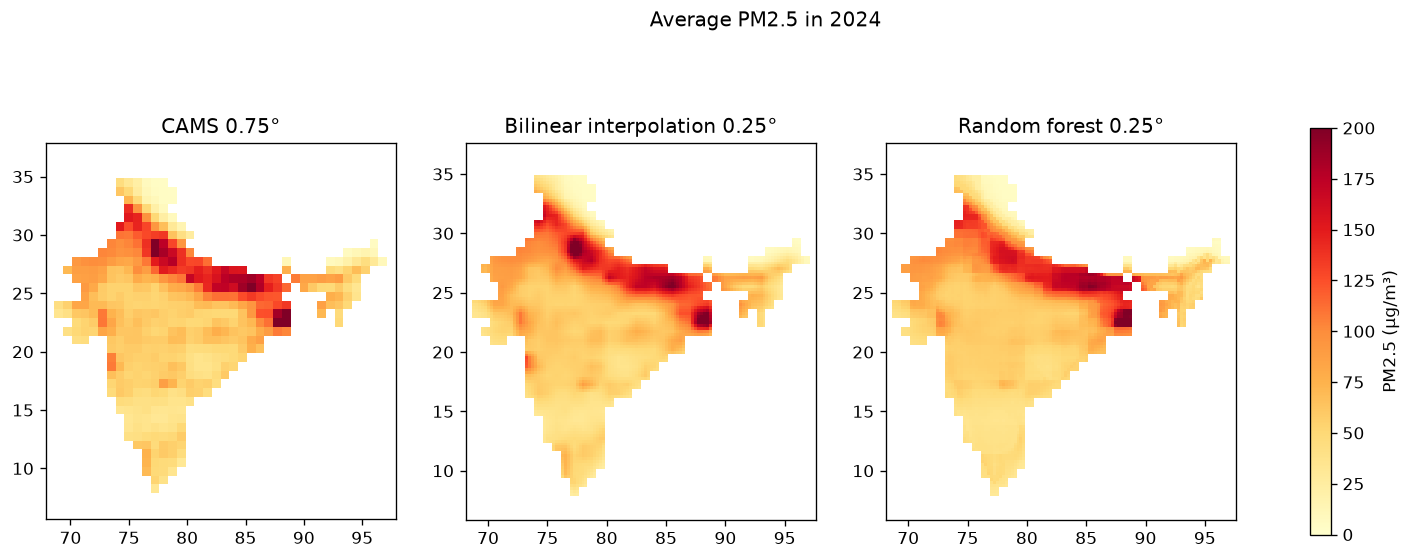
\includegraphics[width=\columnwidth]{figures/map_2024_mean.png}\caption{2024 mean: native CAMS, bilinear 0.25$^\circ$, RF 0.25$^\circ$. Shared color scale in $\mu$g/m$^3$.}\end{figure}
Unweighted grid-point means are 72.80, 72.37 and 71.54~$\mu$g/m$^3$ for CAMS, bilinear and RF. The fine maps differ by 5.41~$\mu$g/m$^3$ on average in absolute terms. Similar global means do not enforce local coarse-grid consistency. No independent high-resolution predictors or measurements establish finer-scale accuracy. The nearest-cell mask approximates boundaries. CAMS agreement does not establish measured exposure accuracy. A single spatial split and temporal correlation limit robustness claims. Further work should evaluate multiple spatial folds, extremes and independent stations.
\section{Conclusion}
RF gives the strongest overall withheld-location agreement among the three methods, with regional exceptions. The notebook and evaluation script reproduce training and held-out scores. A genuine HDF5 archive stores numeric forest state and requires the supplied Python loader; it is not a Keras model. Fine maps implement the requested interpolation-plus-ML workflow while local fine-scale accuracy remains unverified.
\begin{thebibliography}{3}
\bibitem{cams} Copernicus Atmosphere Monitoring Service, ``CAMS global reanalysis (EAC4),'' Atmosphere Data Store. [Online]. Available: \url{https://ads.atmosphere.copernicus.eu/datasets/cams-global-reanalysis-eac4}
\bibitem{breiman} L. Breiman, ``Random forests,'' \emph{Machine Learning}, vol. 45, pp. 5--32, 2001, doi: 10.1023/A:1010933404324.
\bibitem{sklearn} F. Pedregosa \emph{et al.}, ``Scikit-learn: Machine learning in Python,'' \emph{J. Mach. Learn. Res.}, vol. 12, pp. 2825--2830, 2011.
\end{thebibliography}
\end{document}
